\documentclass[]{scrartcl}
\usepackage[utf8]{inputenc}
\usepackage{graphicx}
\usepackage{amsmath}

\title{Formale Simulation und Verifikation verteilter Algorithmen  \\ Abgabe der Praktikumsaufgabe 1}

\author{Maria Lüdemann und Birger Kamp}

\begin{document}

\maketitle

\begin{abstract}

\end{abstract}

\section{Erläuterung der Modellierung}
\begin{figure}[htbp]
	\centering
	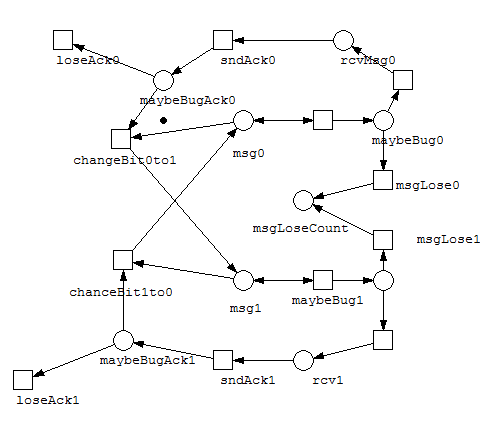
\includegraphics[width=1\linewidth]{altBitPro.png}
	\label{fig:bspModell}
\end{figure}

Diese Modellierung beinhaltet zwei autarke Schleifen die das Senden, eventuelle Verlieren und empfangen der Nachrichten modelieren. Diese Schleife gibt es je für die Nachrichten mit dem Kontrollbit 1 und dem für 0. 

\end{document}
